\documentclass[11pt]{article}
\usepackage[margin=1in]{geometry}                % See geometry.pdf to learn the layout options. There are lots.
\geometry{letterpaper}                   % ... or a4paper or a5paper or ... 
%\geometry{landscape}                % Activate for for rotated page geometry
%\usepackage[parfill]{parskip}    % Activate to begin paragraphs with an empty line rather than an indent
\usepackage{color}
\definecolor{myblue}{rgb}{0.0, 0.0, 0.85}
\usepackage[breaklinks=true, colorlinks=true, linkcolor=red, urlcolor=myblue, citecolor=black]{hyperref}
\urlstyle{rm}
\usepackage{mathptmx}
\usepackage{graphicx}
\usepackage{amssymb}
\usepackage{epstopdf}
\usepackage{sidecap}
\usepackage{authblk}
\usepackage{booktabs}
\usepackage[font=small,labelfont=bf]{caption}
\usepackage{enumitem}
\usepackage{wrapfig}
\usepackage{draftwatermark}
\SetWatermarkText{DRAFT}
\SetWatermarkScale{1.2}
\SetWatermarkColor[gray]{0.85}
\DeclareGraphicsRule{.tif}{png}{.png}{`convert #1 `dirname #1`/`basename #1 .tif`.png}
\pagestyle{plain}

\def\bfr{\bf\color{red}}
\def\bfp{\color{magenta}}
\def\geohub{{\tt geohub}}
\def\resp{respectively}
\def\selah{SELAH}
\def\nch{718}
\def\nh{957\pm94}
\def\dh{10\%\pm9\%}
\def\nce{389}
\def\ne{556\pm83}
\def\de{15\%\pm12\%}

\begin{document}
%\maketitle

\begin{center}
	\Large\bf Mid City West's Unsheltered Population Is Unchanged from 2020\\
	\vspace{1ex}
	{\normalsize\rm Louis Abramson, PhD, and Brian Kohan\\ \today 
	}{\bfr \texttt{ -- NOT FOR DISTRIBUTION}}
\end{center}

\noindent {\bf Summary:} Volunteers surveying Mid City West on March 31, 2021, found  
a non-significant change in adults experiencing unsheltered homelessness compared to the 2020 
LAHSA Count---$7\%\pm15\%$ (90\% CI). A 20\% decline in the number of identified rough 
sleepers was offset by a 95\% increase in the number of tents and makeshift dwellings 
(Figure \ref{fig:rawCounts}). This near-doubling of the most visually salient part of unsheltered 
living would support subjective impressions that the state of homelessness worsened despite the 
total population remaining statistically unchanged. Data from the Coordinated Entry System will 
reveal how changes in sheltered homelessness---perhaps driven by the activation of the Pan Pacific 
Park Rec Center Emergency Shelter---affected Mid City West's total unhoused population.
%As COVID-related contractions in health, sanitation, and social 
%services, have deteriorated conditions on the street, such impressions may yet be accurate. 

\begin{table*}[h]
\caption{Mid City West 2021 Unsheltered Counts and Population Estimates}
\resizebox{\linewidth}{!}{%
\begin{tabular}{lcccccccccc}
\toprule
 & Persons & Car & Van & RV & Tent & Makeshift & {\bf 2021 Total} & {\bf 2020 Total} & {\bf \% change*} \\ \cmidrule{1-10}
Counts & 114 & 6 & 11 & 5 & 49 & 31 & {\bf 219} & {\bf 217} & {\bf $-$1\%}  \\
Inhabitants & 114 (16) & 11 (6) & 20 (8) & 8 (6) & 72 (14) & 52 (13) & {\bf 278 (38)} & {\bf 260} & {\bf 7\% (15\%)}\\
Category share & 41\% (6\%) & 4\% (2\%) & 7\% (3\%) & 3\% (2\%) & 26\% (5\%) & 19\% (5\%) & $-$ & $-$ & $-$
\\ \bottomrule
\end{tabular}
}
\caption*{*Neither the change in raw counts or inferred population is statistically significant (parentheses 
denote 90\% uncertainties). No transition age youth, minors, or families were sighted.}
\label{tbl:summary}
\end{table*}

\begin{figure*}[h]
	\centering
	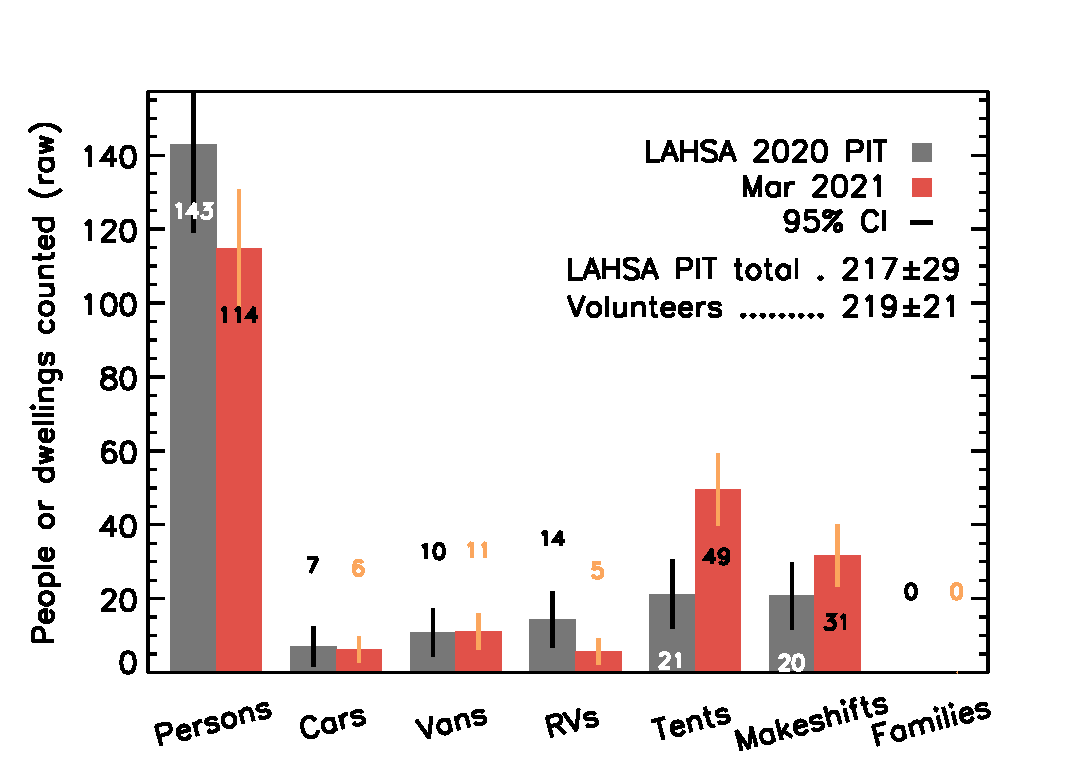
\includegraphics[width = 0.47\textwidth, trim = 1cm 0cm 0cm 1cm]{bars}
	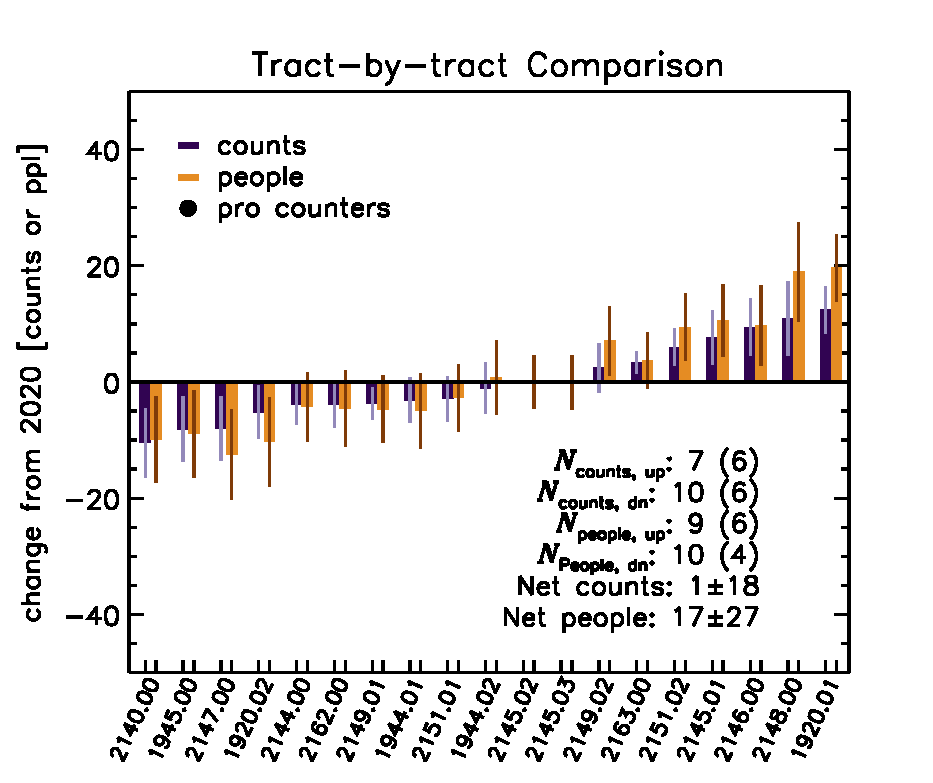
\includegraphics[width = 0.47\textwidth, trim = 0cm 0cm 0cm 1cm]{tractsYrYr.eps}	
	\caption{{\it Left:} total tallies of unsheltered persons + dwellings in Mid City West from 
			the 2020 and 2021 PIT counts (grey/colors). Persons ans RVs fell while 
			tents and perhaps makeshift structures rose. Overall, the same number of 
			people + dwellings were identified as in 2020. {\it Right:} tract-level
			results (see Table \ref{tbl:allTracts}). Compared to 2020, 6 tracts 
			added significantly more unsheltered people, 4 lost them. Tract 2147.00
			at Wilshire/Fairfax saw the largest decline ($-13$ people); 1920.01 along
			the Hollywood border the largest gain ($+20$).}
			%``Persons'' are TAY+Adults.
	\label{fig:rawCounts}
\end{figure*}

%\pagebreak

\noindent {\bf Context:} To compensate for the 
\href{https://laist.com/latest/post/20201209/LAHSA-cancels-2021-homeless-count-los-angeles-covid-19}
{cancellation} of the 2021 LAHSA Count, volunteers in Mid City 
West\footnote{{\bfr ORGS} and resident organizers.} conducted a grassroots enumeration of 
people experiencing unsheltered homelessness 
in all 19 census tracts comprising that community on March 31, 2021 (Figure \ref{fig:tcomp}, top).\\

\begin{wrapfigure}{r}{0.6\linewidth}
	\centering
	\includegraphics[width=\linewidth, trim = 0cm 0cm 0cm 0cm]{map}
	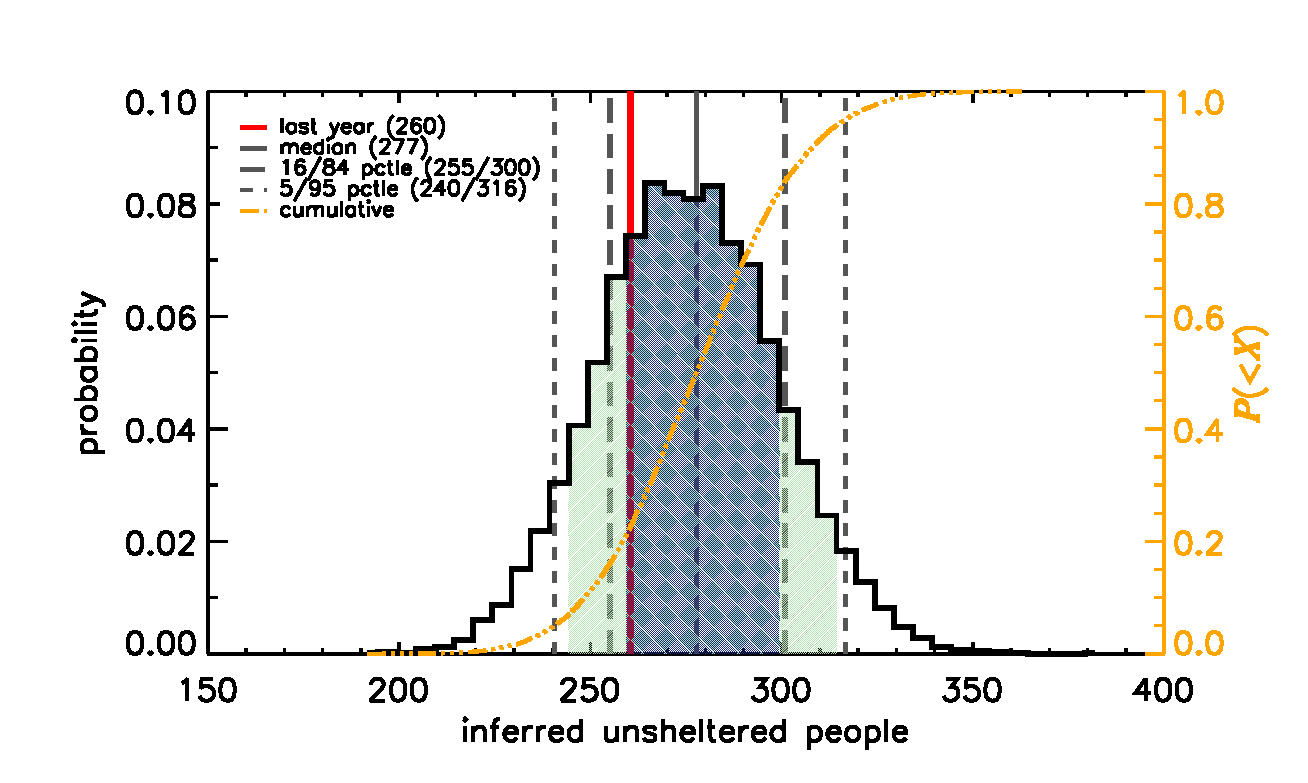
\includegraphics[width=\linewidth, trim = 0cm 0cm 0cm 0cm]{mcw2021Hist}
	\caption{{\it Top:} count area with census tracts colored by  
			changes in unsheltered population from 2020 (red$+$, blue$-$).
			Tracts 2140.00 and 1920.01 saw the largest swings: the former lost
			10 people, the latter gained 20. 
			{\it Bottom:} the probability distribution for Mid City West's total unsheltered 
			population. The median is 7\% above 2020's value, but uncertainties 
			are such that this change is not significant: 22 out of 100 hypothetical surveys
			would have resulted in a population {\it decline} vs.~last year.
			Explore more at \href{https://pit.demoply.org}{pit.demoply.org}.}
	\label{fig:tcomp}
\end{wrapfigure} 

\noindent {\bf Results:} The population estimates in Table \ref{tbl:summary} reflect all 
identified persons, cars, vans, RVs, tents, and makeshift structures with each
dwelling weighted by its average occupancy. These occupancies were set as the area-weighted 
average of those in the LAHSA-defined 
\href{https://www.lahsa.org/documents?id=4686-2020-greater-los-angeles-city-community-homelessness-report-service-planning-area-4.pdf}{communities} of Fairfax (30\%), Mid Wilshire (30\%), and 
Beverly Grove (40\%) from which Mid City West is constituted. Results are unchanged if 
the \href{https://www.lahsa.org/documents?id=4635-usc-2018-2020-multipliers-and-estimates-overview}
{SPA4/CD5} or \href{https://www.lahsa.org/documents?id=4693-2020-greater-los-angeles-homeless-count-cvrtm-conversion-factors}{SPA4-wide} occupancies are used instead, or if the tent weight is 
updated based on a survey performed by {\it The People Concern}.\footnote{Outreach teams 
assessed that 52 people occupied 39 surveyed tents in or around the Mid City West Community,
yielding an estimated $1.33\pm0.18$ people per tent vs.~LAHSA's 2020 value of $1.49\pm0.11$.}

Formally, using Monte Carlo methods, 22 out of 100 simulated Mid City Counts would find an 
unsheltered population lower than 2020's (Figure \ref{fig:tcomp}, bottom). This probability is too high 
compared to the 5/100 benchmark to support claims that the 7\% increase observed in the actual 
Mid City Count is real.

%\begin{wrapfigure}{l}{0.625\linewidth}
%	\centering
%	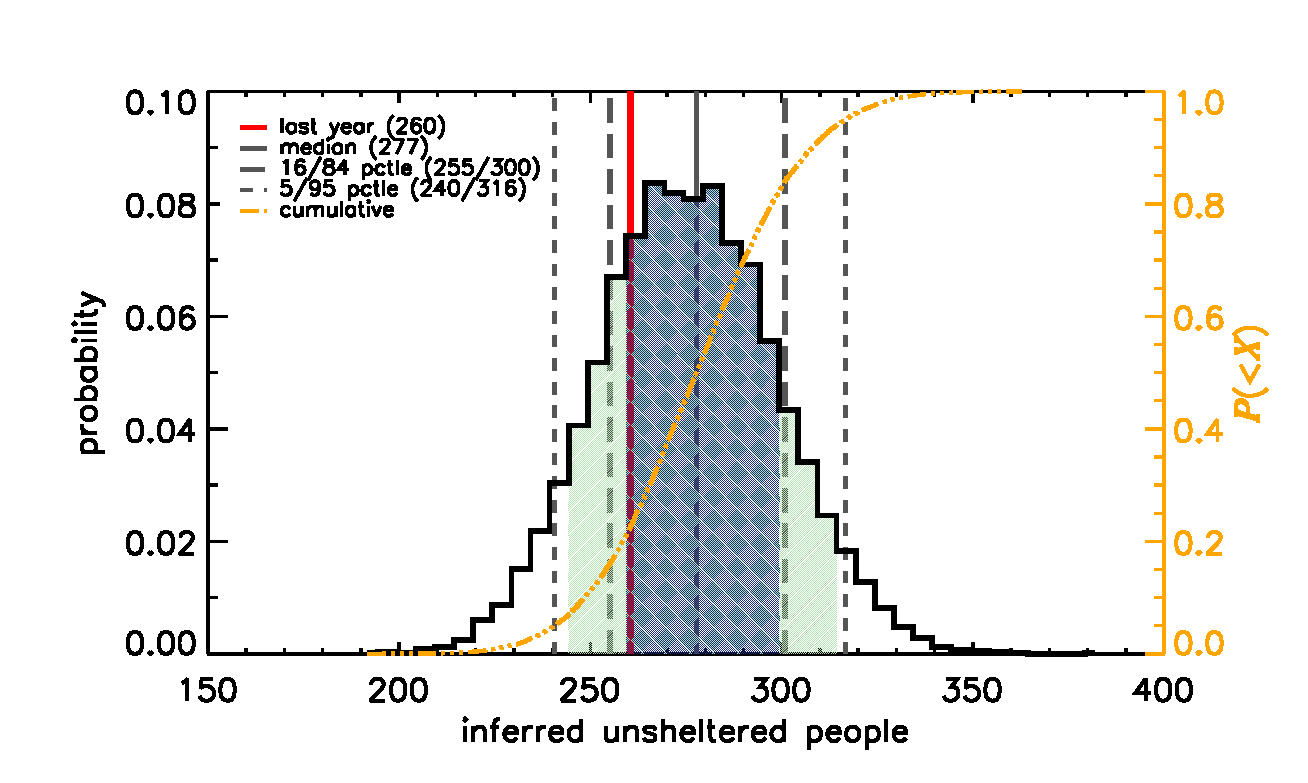
\includegraphics[width=\linewidth, trim = 0cm 0cm 0cm 0cm]{mcw2021Hist}
%	\caption{Probability distributions for the total unsheltered population in Mid City West.}
%	\label{fig:hist}
%\end{wrapfigure} 

Fourteen out of 19 total tracts were counted at least twice (Table \ref{tbl:allTracts}). 
Comparisons of total and per-category results from these independent surveys show visual 
tally errors to be random, as the analysis assumes. The count uncertainty is $\pm$10\% (95\% CI), 
with the remainder of the $\pm$15\% total population margin of error due to the range in 
dwelling occupancies.\\

\noindent {\bf Comments:} These results reflect a $\sim$20\% drop in the number
of adult individuals seen on the street---mirroring trends in neighboring 
\href{https://www.latimes.com/homeless-housing/story/2021-04-13/despite-appearances-15-fewer-homeless-people-were-on-hollywood-streets-this-year}{Hollywood}---offset by a doubling in tents and 
makeshift structures. Government initiatives to stop evictions and move people indoors may be 
responsible. If \href{https://www.lahsa.org/documents?id=4664-2020-homeless-count-council-district-5}{CD5's} 3.4\% share of \href{https://www.lahsa.org/documents?id=4585-2020-greater-los-angeles-homeless-count-los-angeles-continuum-of-care-coc-}{LA County's unsheltered seniors} 
is an indication, 60 CD5 residents might have been in any of Project Roomkey's 
\href{https://projectroomkeytracker.com/}{1770 active rooms} on the night of the count. Others
may have been in Pan Pacific Park's COVID-activated emergency beds. Coordinated Entry System data 
will show if the above scenarios are true.

If there are no fewer people on the street compared to 2020, their quality of life has worsened. \begin{wraptable}{r}{0.55\linewidth}
%\begin{table}[t]
\caption{Census Tract-level Unsheltered Data}
%\resizebox{\textwidth}{!}{%
\centering
\begin{tabular}{ccccc}
\toprule
Tract & Counter & Passes & Median Est. & 90\% CI \\ \cmidrule{1-5}
1920.01 & Vol & 3 & 29 & 21--37 \\
1920.02 & Vol & 2 & 13 & 5--20 \\
1944.01 & Vol & 2 & 10 & 2--17 \\
1944.02 & Vol & 2 & 16 & 8--23 \\
1945.00 & Vol & 2 & 19 & 10--26 \\
2140.00 & Vol & 2 & 19 & 11--27 \\
2144.00 & Vol & 2 & 6 & 0--14 \\
2145.01$^{\rm a}$ & Pro/Vol & 2 & 24 & 15--31 \\
2145.02$^{\rm b}$  & Vol & 1 & 0 & 0--7 \\
2145.03$^{\rm b}$  & Vol & 1 & 0 & 0--7 \\
2146.00 & Vol & 2 & 27 & 19--34 \\
2147.00 & Vol & 1 & 12 & 3--19 \\
2148.00 & Vol & 2 & 46 & 36--56 \\
2149.01 & Vol & 3 & 4 & 0--11 \\
2149.02 & Vol & 2 & 19 & 10--26 \\
2151.01 & Vol & 1 & 7 & 0--14 \\
2151.02 & Vol & 1 & 11 & 2--20 \\
2162.00 & Vol & 2 & 10 & 2--18 \\
2163.00 & Vol & 3 & 6 & 0--13 \\
\cmidrule{1-5}
{\bf All} & & {\bf 36} & {\bf 277} & {\bf 240--316}
\\ \bottomrule
\end{tabular}
%}
\caption*{$^{\rm a}$Tract counted by professional outreach teams
31 March and volunteers 14 April; contains Pan Pacific Park and emergency 
shelter. $^{\rm b}$Park La Brea gated community counted 11 April.}
\label{tbl:allTracts}
%\end{table}
\end{wraptable}COVID has restricted or eliminated access to restaurant bathrooms, libraries 
(\href{https://www.lapl.org/homeless-resources/the-source}{\it The Source}), DPSS 
(EBT, Medi-Cal), DMV (IDs), and DMH facilities. Physical limits on client access at 
hospitals has also kept caseworkers from managing successful discharges. These harms 
are reflected by a 25\% increase in 
\href{https://www.latimes.com/california/story/2021-01-07/the-powerful-synthetic-opioid-fentanyl-is-behind-rising-deaths-in-the-homeless-population}{overdose deaths} and made more visible by \href{https://clkrep.lacity.org/onlinedocs/2020/20-0147_misc_3-17-20_p.pdf}{suspended}
tent folding and sanitation practices as tents increased significantly. 
Of course, no drop in unsheltered homelessness implies substantial coming challenges
 \href{https://www.latimes.com/california/story/2021-01-12/new-report-foresees-tens-of-thousands-losing-homes-by-2023}{as eviction moratoria lapse}.

The data support the effectiveness of programs aimed at curbing a rise in street homelessness.
Yet, they do {\it not} suggest that the state of homelessness has improved. In the fight to rebuild 
lives as we build homes, that fact must remain paramount.

%\clearpage

\end{document}  